
\documentclass[11pt,a4paper]{article}
\usepackage[T1]{fontenc}
\usepackage[T1,hyphens]{url}
\usepackage{amsfonts, amsmath, amssymb}
%\usepackage{showlabels}
%\usepackage{todonotes}
\usepackage{float}
\usepackage{parskip}
\usepackage{graphicx}
\newtheorem{definition}{Definition}
\newtheorem{theorem}{Theorem}
\newtheorem{postulate}{Postulate}
\newtheorem{lemma}{Lemma}
\newtheorem{comment}{Comment}
\newtheorem{proposition}{Proposition}
\newtheorem{corollary}{Corollary}
\newtheorem{fact}{Fact}
\newtheorem{remark}{Remark}
\newtheorem{example}{Example}
\newenvironment{proof}{\textsf{\bfseries{}Proof. }}{\qed\par}
\usepackage{algorithm}
\usepackage{algpseudocode}
%%%%%%%%%%%%%%%%%

 \newcommand{\bbbn}{\mathbb{N}}
 \newcommand{\bbbz}{\mathbb{Z}}
 \newcommand{\bbbq}{\mathbb{Q}}
 \newcommand{\bbbr}{\mathbb{R}}
 \newcommand{\bbbc}{\mathbb{C}}
 \newcommand{\II}{\mathbf{I}}
 \newcommand{\dom}{\mathrm{dom}}
 \newcommand{\w}{\mathbf{w}}
 \newcommand{\x}{\mathbf{x}}
 \newcommand{\rr}{r}
 \newcommand{\la}{\lambda}
 \newcommand{\CONV}{\Gamma}
 \newcommand{\f}{\varphi}
 \newcommand{\de}{\delta}
 \newcommand{\al}{\alpha}
 \newcommand{\be}{\beta}
 \newcommand{\e}{\in}
 %\newcommand{\v}{\mathbf{v}}
 \newcommand{\s}{\rightarrow}
 \newcommand{\y}{\mathbf{y}}
 \newcommand{\z}{\mathbf{z}}
 \newcommand{\COM}[2]{{#1 \choose #2}}
 \newcommand{\mg}{\mbox{mg}}
\newcommand{\Tr}{\mathrm{Tr}}
%%%%%%%%%%%%%%%%%
\usepackage{verbatim}
\usepackage{enumerate}

%%%%%%%%%%%%%%%%%

\usepackage{physics}
%\newcommand{\ket}[1]{| #1 \rangle}
%\newcommand{\bra}[1]{\langle #1 |}
\newcommand{\bracket}[2]{\langle #1| #2 \rangle}
 \newcommand{\iprod}[2]{\langle #1 | #2 \rangle}
 \newcommand{\mprod}[3]{\langle #1 | #2 | #3 \rangle}
 \newcommand{\oprod}[2]{| #1 \rangle\langle #2 |}
 \newcommand{\qed}{\mbox{ }\hfill$\square$\par}

%%%%%%%%%%%%%%%%%

%\usepackage[backref=page,pagebackref=true,linkcolor = blue,citecolor = red]{hyperref}
%\usepackage[backref=page]{backref}
%\newcommand{\chapquote}[3]{\begin{quotation} \textit{#1} \end{quotation}

%%%%%%%%%%%%%%%%%

\usepackage{times}
\usepackage{sectsty}
\usepackage{xcolor,colortbl}
\usepackage[framemethod=tikz]{mdframed}
\usepackage{caption}
\usepackage{adjustbox}
\usepackage{systeme}
\usepackage{multicol}
\usepackage{graphicx}

%%%%%%%%%%%%%%%%%

 %\begin{flushright} - #2, \textit{#3}\end{flushright} }

  %%%%%%%%%%%%%%%%%


 %%%%%%%%%%%%%%%%%

\begin{document}

\title{Three-Dimensional Quantum Random Generator: Theory, Realisation and Testing or\\
Suplementary Material to ``How Real Is Incomputability in Physics''???}
\author{Jos\'{e} Manuel Ag\"{u}ero$^{1}$
         Trejo, Cristian S. Calude$^{1}$
         Michael J. Dinneen$^{1}$,\\
         Arkady Fedorov$^{2,3}$, Anatoly Kulikov$^{2,3}$, Rohit Navarathna$^{2,3}$, Karl Svozil$^{4}$\\[3ex]$^{1}$School of Computer Science, University of Auckland, New Zealand\\
         $^{2}$School of Mathematics and Physics, University of Queensland, Australia\\
         $^{3}$ARC Centre of Excellence for Engineered Quantum Systems, Queensland, Australia\\
         $^{4}$Institute f\"ur Theoretische Physik, TU Wien, Vienna, Austria}
\date{\today}


\maketitle

\begin{abstract}
Something
\end{abstract}

\cite{PhysRevLett.119.240501,Abbott_2019}
\section{Introduction}

There are several methods to generate quantum randomness, among them radioactive decay~\cite{Kohlrausch1926,Kragh-2009_RePoss5},
diodes, as well as quantum coin tosses~\cite{svozil-qct,zeilinger:qct,Quantis}.
In what follows we shall concentrate on the latter type of quantum random number generators from generalized beam splitters~\cite{rzbb},
with the additional benefit of certification relative to quantum contextuality~\cite{svozil-2009-howto,10.1038/nature09008}.

Thereby, the (meta)physical message---rather a hypothesis---according
to one of the current nobel prize winners in physics is that of irreducible randomness~\cite{zeil-05_nature_ofQuantum}:
 \begin{quote}
$\ldots$~for the individual event in quantum physics, not only do we not know the cause, there is no cause.
 \end{quote}
The essential feature of quantum randomness resides in its ontological {\em underdetermination},
as compared to epistemic, subjective but not objective~\cite{Heisenberg1958-HEIPAP}
uncertainty reducible to ignorance of classical physical states and evolution, even in the case of chaotic behaviour.

Quantum underdetermination can be expressed in terms of gaps in the physical description~\cite[\S~III.12-14]{frank,franke}:
due to the unitarity of the quantum evolution information cannot be created nor annihilated.
Therefore, if a quantized system encodes a finite amount of information any query in excess of this information
must inevitably be indeterminate and value indefinite relative to the original quantum state.
One could, of course, suppose that such a request can be fulfilled by the entanglement
with the measurement apparatus and thus the environment at large~\cite{london-Bauer-1939,london-Bauer-1983}, resulting in an
unbounded nesting argument with an ever increasing Heisenberg cut.
Yet the fact remains that, due to the finite (possibly relational~\cite{zeil-99}) amount of information encoded in a quantized system,
information in excess of this amount cannot reside or be encoded in any pre-selected state.

Underdetermination gets also expressed in the Kochen-Specker theorem and other configurations of observables with a scarcity
of two-valued states associated with simultaneous classical truth assignments~\cite[Theorem~0]{kochen2}.
This is also true for Boole's conditions of possible experience
in non-local configurations under strict Einstein causality~\cite{wjswz-98,Zeilinger2005-kj,Zeilinger2007-mm}.

As a result the current quantum canon can charactrized in theological, scholastic terms as {\it Creatio Continua},
the continuous creation of randomness on a massive scale.
Another alternative is the postulate of non-local hidden parameters; an assumption that lacks any current empirical basis.

\section{3D QRNG -- Theory}
The 3D QRNG constructs a value-indefinite observable and then measures it, in a repetitive manner;
the probability distribution of the outcomes is $1/4, 1/2,1/4$.

In this section we present the theoretical framework allowing the construction of value-indefinite observables, their tolerance to measurement errors and the certification of the degree of randomness of their outcomes.


\subsection{Notation and definitions}
\label{notat}
The set of positive integers will be denoted by $\bbbn$. Consider the alphabet
$A_{b}=\{0,1,\dots ,b-1\}$, where $b\ge 2$ is an integer; the elements of
$A_b$ are to be considered the digits used in natural positional
representations of numbers in the interval $[0,1)$ at base $b$. By  $A_{b}^{*}$
and  $A_{b}^{\omega}$ we denote the sets of (finite)  strings and (infinite)
sequences over the alphabet $A_{b}$. Strings will be denoted by $x,y,u,w$; the
length of the string $x= x_1x_2\dots x_m$, $x_i\in A_{b}$, is denoted by
$|x|_{b}=m$ (the subscript $b$ will be omitted if it is clear from the
context); $A_{b}^{m}$ is the set of all strings of length $m$.  Sequences will
be denoted by $\mathbf{x}= x_1x_2\dots$; the prefix of length $m$ of
$\mathbf{x}$ is the string $ \mathbf{x}(m)= x_1x_2\dots x_m$.
Strings
will be ordered quasi-lexicographically according to the natural order $0<1<2  < \dots <b-1$ on the
alphabet $A_{b}$. For example, for $b=2$, we have $0<1<00<01<10<11<000 \dots$.
We
assume knowledge of elementary computability theory over different size
alphabets~\cite{calude:02}.

By $\mathbb{C}$ we denote the set of complex numbers.
%Sequences can be also viewed as $A_{b}$-valued functions defined on $\bbbn$.
We then fix a positive integer $n\geq 2$ and let $O \subseteq \{  P_{\psi}:  \ket{\psi} \in \mathbb{C}^{n} \}$ be a non-empty set of one-dimensional projection observables on the Hilbert space $\mathbb{C}^{n}$.


A set $C \subset O$ is a {\it  context} of $O$ if $C$ has $n$ elements  and for all $P_{\psi}, P_{\phi} \in C$ with $P_{\psi} \neq P_{\phi}, \braket{\psi}{\phi} = O$.
A  {\it  value assignment function} (on $O$) is a partial function $v:O\to \{0,1\}$ assigning values to some (possibly all) observables in $O$.  The partiality of the  function $v$ means that $v(P)$ can be $0,1$ or indefinite.
An observable $P \in O$ is  {\it  value definite} (under the assignment function $v$)  if $v(P)$ is defined, i.e.~it is 0 or 1; otherwise, it is  {\it  value indefinite} (under $v$). Similarly, we call $O$  {\it  value definite} (under $v$) if every observable $P \in O$ is value definite.


We then fix a positive integer $n\geq 2$ and let $O \subseteq \{  P_{\psi}:  \ket{\psi} \in \mathbb{C}^{n} \}$ be a non-empty set of one-dimensional projection observables on the Hilbert space $\mathbb{C}^{n}$.
A set $C \subset O$ is a {\it  context} of $O$ if $C$ has $n$ elements and for all $P_{\psi}, P_{\phi} \in C$ with $P_{\psi} \neq P_{\phi}, \braket{\psi}{\phi} = O$.
A  {\it  value assignment function} (on $O$) is a partial function $v:O\to \{0,1\}$ assigning values to some (possibly all) observables in $O$.  The partiality of the  function $v$ means that $v(P)$ can be $0,1$ or indefinite.
An observable $P \in O$ is  {\it  value definite} (under the assignment function $v$)  if $v(P)$ is defined, i.e.~it is 0 or 1; otherwise, it is  {\it  value indefinite} (under $v$). Similarly, $O$ is {\it  value definite} (under $v$) if every observable $P \in O$ is value definite.
%(a pre-existing physical property)



\subsection{Localised Kochen-Specker Theorem}
We next present the main result used to construct a value indefinite observable. First, we assume  the following  premises:

\begin{itemize}
\item {\bf Admissibility.} Fix a set $O$  of one-dimensional projection observables on $\mathbb{C}^{n}$ and the value assignment function $v:O\rightarrow \{0,1\}$. Then $v$ is  {\it  admissible} if for  every context $C$ of $O$, we have that $\sum_{P\in C}v(P) = 1$.
This condition postulates that only one projection observable in a context can be assigned the value $1$. This gurantees the agreement with quantum mechanics predictions.
 %$v$ is a Boolean frame function with weight $1$, so



\item {\bf Non-contextuality of definite values.}  Every outcome obtained by
measuring a value definite observable
 is {\it  non-contextual}, i.e.\ it does not
depend on other compatible
 observables which may be measured alongside it.
 \item{\bf Eigenstate principle.}  If a quantum system is prepared in the
state $\ket{\psi}$, then the projection observable
$P_\psi$ is value definite.
\end{itemize}

The last assumption is motivated by  Einstein, Podolsky and Rosen  definition of {\em physical reality}~\cite[p.~777]{epr}:

 \begin{quote}
         If, without in any way disturbing a system, we can predict with certainty the value of a physical quantity, then there exists a \emph{definite value} prior to observation corresponding to this physical quantity.
\end{quote}
It gives a criterion for value-definitiness: if a quantum system is prepared in an arbitrary state $\ket{\psi}\in\mathbb{C}^{n}$, then the measurement of the observable $P_{\psi}$ should yield the outcome $1$, hence, if $P_{\psi}\in O$, then $v(P_{\psi})=1.$

We can state now main result:


\begin{theorem}[Localised Kochen-Specker Theorem~\cite{Abbott:2010uq,acs-2015-info6040773,PhysRevLett.119.240501, aguero_trejo_new_2021}]
\label{EffecKS}
        Assume a quantum system prepared in the state
$\ket{\psi}$ in a dimension $n\ge 3$ Hilbert space ${\mathbf C}^n$, and let $\ket{\phi}$
be any quantum state such that  $0<\abs{\bra{\psi}\ket{\phi}}<1$. If the following three conditions are satisfied: i) admissibility, ii) non-contextuality and iii)
eigenstate principle,
then the projection observable $P_\psi$ is  value
indefinite.
\end{theorem}


Theorem~\ref{EffecKS} states that, under the given assumptions,  any quantum state $\ket{\phi}$ that is  neither orthogonal nor parallel to $\ket{\psi}$ is {\it value indefinite}. This result has two major consequences:

\begin{enumerate}
    \item it shows how to effectively construct a value indefinite observable, and
    \item it guarantees that the status of ``value-indefiniteness'' is invariant under the small errors in measurements: this is a very important property as no measurement is exact.
\end{enumerate}



How ``good'' is such a 3D QRNG, i.e.~what randomness properties can be {\it certified} for their outcomes?  For example, can we prove that the outcomes of the 3D QRNG are ``better'' than the outcomes produced by {\it any} pseudo-random number generator (PRNG)?

We note that Theorem~\ref{EffecKS}, as the original Kochen-Specker Theorem, is not true in ${\mathbf C}^2$~\cite{kochen1}, so the requirement to work in ${\mathbf C}^3$.

For certification we use the following new assumption:


\begin{itemize}
        \item  {\bf epr  principle}: If a repetition of measurements of an
observable generates a computable sequence, then  these observables
are value definite.
\end{itemize}

Based on  the  Eigenstate and epr    principles we can prove that the answer to the last question is affirmative. Any infinite repetition of the
experiment
measuring  a quantum value indefinite observable generates an
incomputable   infinite sequence $x_1x_2\dots$: no PRNG has this randomness property.


A stronger result is in fact true. Informally, a sequence $ \mathbf{x}$ is bi-immune if  no algorithm can generate
infinitely many correct values of its elements (pairs, $(i, x_i)$).
Formally, a.
 sequence $ \mathbf{x}\in A_{b}^{\omega}$  ($b\ge 2$)
 is  {\it bi-immune} if there is no
partially computable function $\varphi$ from $\bbbn $ to $A_{b}$ having an
infinite domain $\dom(\varphi)$ with the property that $\varphi(i)= x_i$ for
all $i\in \dom(\varphi)$~\cite{bienvenu2013}).


\begin{theorem}[\cite{abbott2012strongrandomness,aguero_trejo_new_2021}]
\label{biimm_2}
Assume the  Eigenstate and epr    principles. An infinite repetition of the
experiment
measuring  a quantum value indefinite observable  in $\mathbb{C}^{b}$ always generates a
 $b$-bi-immune   sequence $\x\in A_2^{\omega}$, for every $b\ge 2$.
\end{theorem}

In particular, every sequence generated by the 3D QRNG is 3-bi-immune.

\begin{theorem}  [\cite{aguero_trejo_new_2021}]
\label{bunpredict}
Assume the epr and Eigenstate  principles.
Let $\x$ be an infinite sequence obtained by measuring  a quantum value indefinite observable  in $\mathbb{C}^{b}$  in an infinite repetition of the experiment $E$. Then no single bit $x_i$ can be predicted.
\end{theorem}

In particular, no single digit of every  sequence   $\x \in A_3^{\omega}$ generated by the 3D QRNG  can be algorithmically predicted.

The following simple morphism $\varphi \colon A_3 \rightarrow A_2$ transforms a ternary
sequence into a binary sequence:

\begin{equation}
\label{amorph}
\varphi(a)=
\begin{cases}0,&\text{if }a=0,
\\1,&\text{if }a=1,
\\0&\text{if } a=2,\end{cases}
\end{equation}



\noindent  which can be extended sequentially for strings,
  $\mathbf{y}(n)=\varphi(\mathbf{x}(n))= \varphi(x_1)\varphi(x_2)$  $\dots \varphi(x_n)$ and sequences $\mathbf{y}= \varphi(\mathbf{x}) = \varphi(x_1)\varphi(x_2)\dots \varphi(x_n) \dots $. This transformation preserves 2-bimmunity:

  \begin{theorem}[\cite{aguero_trejo_new_2021}]
        Assume the epr and Eigenstate  principles. Let $\mathbf{y}=\varphi (\mathbf{x})$, where $\mathbf{x}\in A_3^{\omega}$ is a ternary sequence generated by the  QRNG  and $\varphi$ is the alphabetic morphism defined in (\ref{amorph}).
Then, no single bit of    $\y \in A_2^{\omega}$  can be predicted.
\end{theorem}



%Finally, we present the formal framework of the measurement of a valued-indefinite observable used by the 3D QRNG.

As noted in~\cite{aguero_trejo_new_2021},  Theorem~\ref{EffecKS} shows that, given a system prepared in state $\ket{\psi}$, a one-dimensional projection observable can only be value definite if it is an eigenstate of that observable. Consequently,  for any diagonalisable observable $O$ with spectral decomposition $O=\sum_{i=1}^n\lambda_{i}P_{\lambda_{i}}$, where $\lambda_{i}$ denotes each distinct eigenvalue with corresponding eigenstate $\ket{\lambda_{i}}$,  $O$ has a predetermined measurement outcome if and only if each projector in its spectral decomposition has a predetermined measurement outcome. Thus,  the  previous result holds true  to the outcome of the measurement of any observable with non-degenerate spectra.
Such generalisation is  particularly useful in the case when we use the value assignment function to represent  a  value definite observable.
These results have been used  to design the following quantum operators of the 3D QRNG.  These QRNGs operate in a  succession of events of the form ``preparation,  measurement,
 reset'', iterated indefinitely many times in an algorithmic fashion~\cite{abbott2012strongrandomness}. The first 3D QRNG was designed in~\cite{abbott2012strongrandomness}, realized in~\cite{PhysRevLett.119.240501} and analysed in~\cite{Abbott_2019}. While the analysis failed to observe a strong advantage of the quantum random sequences due to incomputability, it has motivated the improvement in ~\cite{aguero_trejo_new_2021}, in which  the problematic probability zero  branch  $S_x=0$  in Figure~\ref{fig1}.

\begin{figure}[ht]
\centering
\tikzset{every picture/.style={line width=0.60pt}} %set default line width to 0.75pt
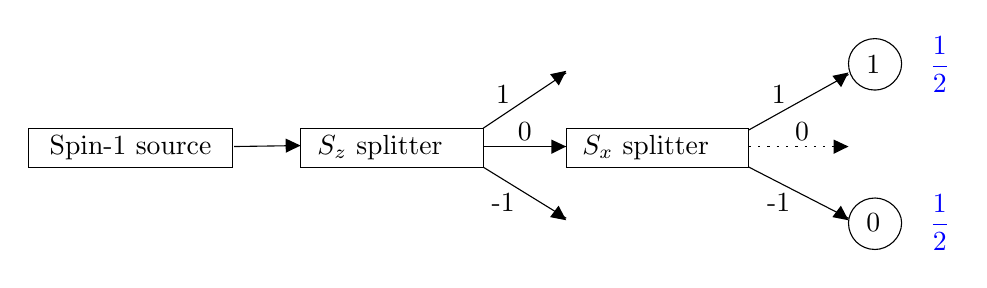
\begin{tikzpicture}[x=0.6pt,y=0.6pt,yscale=-1,xscale=1]
\draw   (26,129) -- (149.2,129) -- (149.2,152.4) -- (26,152.4) -- cycle ;
\draw    (150,140) -- (190,139.42) ;
\draw [shift={(190,139.4)}, rotate = 539.51] [fill={rgb, 255:red, 0; green, 0; blue, 0 }  ][line width=0.75]  [draw opacity=0] (8.93,-4.29) -- (0,0) -- (8.93,4.29) -- cycle    ;
\draw   (190,129) -- (300,129) -- (300,152.4) -- (190,152.4) -- cycle ;
\draw    (300,140) -- (350,140) ;
\draw [shift={(350,140)}, rotate = 539.51] [fill={rgb, 255:red, 0; green, 0; blue, 0 }  ][line width=0.75]  [draw opacity=0] (8.93,-4.29) -- (0,0) -- (8.93,4.29) -- cycle    ;
\draw   (350,129) -- (460,129) -- (460,152.4) -- (350,152.4) -- cycle ;
\draw [dash pattern={on 0.84pt off 2.51pt}](460,140) -- (520,140) ;
\draw [shift={(520,140)}, rotate = 539.51] [fill={rgb, 255:red, 0; green, 0; blue, 0 }  ][line width=0.75]  [draw opacity=0] (8.93,-4.29) -- (0,0) -- (8.93,4.29) -- cycle    ;
\draw    (300,152.4) -- (350,183.21) ;
\draw [shift={(350,184.4)}, rotate = 216.66] [fill={rgb, 255:red, 0; green, 0; blue, 0 }  ][line width=0.75]  [draw opacity=0] (8.93,-4.29) -- (0,0) -- (8.93,4.29) -- cycle    ;
\draw    (300,129) -- (350,95.62) ;
\draw [shift={(350,94.4)}, rotate = 502.44] [fill={rgb, 255:red, 0; green, 0; blue, 0 }  ][line width=0.75]  [draw opacity=0] (8.93,-4.29) -- (0,0) -- (8.93,4.29) -- cycle    ;
\draw    (460,130) -- (520,96.62) ;
\draw [shift={(520,95.4)}, rotate = 502.44] [fill={rgb, 255:red, 0; green, 0; blue, 0 }  ][line width=0.75]  [draw opacity=0] (8.93,-4.29) -- (0,0) -- (8.93,4.29) -- cycle    ;
\draw    (460,152.4) -- (520,183.21) ;
\draw [shift={(520,184.4)}, rotate = 216.66] [fill={rgb, 255:red, 0; green, 0; blue, 0 }  ][line width=0.75]  [draw opacity=0] (8.93,-4.29) -- (0,0) -- (8.93,4.29) -- cycle    ;
\draw   (520,90) .. controls (520,82) and (527,75) .. (536,75) .. controls (544,75) and (552,82) .. (552,90) .. controls (552,99) and (544,106) .. (536,106) .. controls (527,106) and (520,99) .. (520,90) -- cycle ;
\draw   (520,186) .. controls (520,178) and (527,171) .. (536,171) .. controls (544,171) and (552,178) .. (552,186) .. controls (552,195) and (544,202) .. (536,202) .. controls (527,202) and (520,195) .. (520,186) -- cycle ;
\draw (87.6,140.7) node  [align=left] {Spin-1 source};
\draw (240.6,140.7) node  [align=left] {$\displaystyle S_{z}$ splitter };
\draw (400.6,140.7) node  [align=left] {$\displaystyle S_{x}$ splitter };
\draw (312,109) node  [align=left] {1};
\draw (312,174) node  [align=left] {\mbox{-}1};
\draw (325,131) node  [align=left] {0};
\draw (535,90.7) node  [align=left] {1};
\draw (535,185.7) node  [align=left] {0};
\draw (478,109) node  [align=left] {1};
\draw (478,174) node  [align=left] {\mbox{-}1};
\draw (492,131) node  [align=left] {0};
\draw (575,90.7) node  [align=left] {$\displaystyle\color{blue}{\frac{1}{2}}$};
\draw (575,185.7) node  [align=left] {$\displaystyle\color{blue}{\frac{1}{2}}$};
\end{tikzpicture}
\caption{QRNG setup proposed in \cite{abbott2012strongrandomness}; the values $\frac{1}{2},\frac{1}{2}$ (in blue) correspond to the outcome probabilities}
\label{fig1}
\end{figure}

The next 3D QRNG is presented in
Figure~\ref{fig2}. The unitary matrix $U_{x}$ corresponding to the spin state operator $S_x$ is
 $$ U_x = \frac{1}{2}
 \begin{pmatrix}
 1 & \sqrt{2} & 1\\
 \sqrt{2} & 0 & -\sqrt{2}\\
 1 & -\sqrt{2} & 1
 \end{pmatrix}.$$

As  $U_x$ can be decomposed into two-dimensional transformations~\cite{Clements:16}

$$U_x =
\begin{pmatrix}1&0&0\\
0&-i&0\\
0&0&-i
\end{pmatrix}
\cdot
\begin{pmatrix}
\frac{1}{\sqrt{3}} & \sqrt{\frac{2}{3}} & 0\\
i\sqrt{\frac{2}{3}} & -\frac{i}{\sqrt{3}} & 0\\
0&0&1\\
\end{pmatrix}
\cdot
\begin{pmatrix}
\frac{\sqrt{3}}{2} & 0 & -\frac{i}{2}\\
0&1&0\\
\frac{i}{2}& 0 & -\frac{\sqrt{3}}{2}\\
\end{pmatrix}
\cdot
\begin{pmatrix}
1&0&0\\
0&\frac{1}{\sqrt{3}} &\sqrt{\frac{2}{3}}\\
0 & i\sqrt{\frac{2}{3}} & -\frac{i}{\sqrt{3}}
\end{pmatrix}.
$$

a physical realisation of the unitary operator by a lossless beam splitter~\cite{PhysRevLett.73.58,yurke-86} was obtained;  the new outcome probabilities are 1/4,1/2,/1/4.


\begin{figure}
\centering
\tikzset{every picture/.style={line width=0.60pt}} %set default line width to 0.75pt
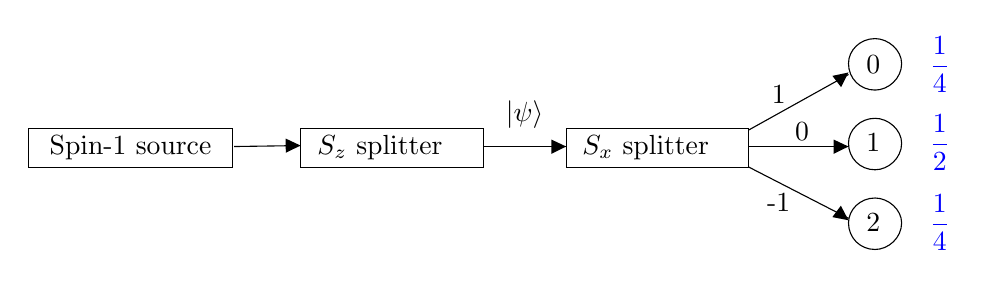
\begin{tikzpicture}[x=0.6pt,y=0.6pt,yscale=-1,xscale=1]
\draw   (26,129) -- (149.2,129) -- (149.2,152.4) -- (26,152.4) -- cycle ;
\draw    (150,140) -- (190,139.42) ;
\draw [shift={(190,139.4)}, rotate = 539.51] [fill={rgb, 255:red, 0; green, 0; blue, 0 }  ][line width=0.75]  [draw opacity=0] (8.93,-4.29) -- (0,0) -- (8.93,4.29) -- cycle    ;
\draw   (190,129) -- (300,129) -- (300,152.4) -- (190,152.4) -- cycle ;
\draw    (300,140) -- (350,140) ;
\draw [shift={(350,140)}, rotate = 539.51] [fill={rgb, 255:red, 0; green, 0; blue, 0 }  ][line width=0.75]  [draw opacity=0] (8.93,-4.29) -- (0,0) -- (8.93,4.29) -- cycle    ;
\draw   (350,129) -- (460,129) -- (460,152.4) -- (350,152.4) -- cycle ;
\draw (460,140) -- (520,140) ;
\draw [shift={(520,140)}, rotate = 539.51] [fill={rgb, 255:red, 0; green, 0; blue, 0 }  ][line width=0.75]  [draw opacity=0] (8.93,-4.29) -- (0,0) -- (8.93,4.29) -- cycle    ;
\draw    (460,130) -- (520,96.62) ;
\draw [shift={(520,95.4)}, rotate = 502.44] [fill={rgb, 255:red, 0; green, 0; blue, 0 }  ][line width=0.75]  [draw opacity=0] (8.93,-4.29) -- (0,0) -- (8.93,4.29) -- cycle    ;
\draw    (460,152.4) -- (520,183.21) ;
\draw [shift={(520,184.4)}, rotate = 216.66] [fill={rgb, 255:red, 0; green, 0; blue, 0 }  ][line width=0.75]  [draw opacity=0] (8.93,-4.29) -- (0,0) -- (8.93,4.29) -- cycle    ;
\draw   (520,90) .. controls (520,82) and (527,75) .. (536,75) .. controls (544,75) and (552,82) .. (552,90) .. controls (552,99) and (544,106) .. (536,106) .. controls (527,106) and (520,99) .. (520,90) -- cycle ;
\draw   (520,138) .. controls (520,130) and (527,123) .. (536,123) .. controls (544,123) and (552,130) .. (552,138) .. controls (552,147) and (544,154) .. (536,154) .. controls (527,154) and (520,147) .. (520,138) -- cycle ;
\draw   (520,186) .. controls (520,178) and (527,171) .. (536,171) .. controls (544,171) and (552,178) .. (552,186) .. controls (552,195) and (544,202) .. (536,202) .. controls (527,202) and (520,195) .. (520,186) -- cycle ;
\draw (87.6,140.7) node  [align=left] {Spin-1 source};
\draw (240.6,140.7) node  [align=left] {$\displaystyle S_{z}$ splitter };
\draw (400.6,140.7) node  [align=left] {$\displaystyle S_{x}$ splitter };
\draw (325,121) node  [align=left] {$\ket{\psi}$};
\draw (535,90.7) node  [align=left] {0};
\draw (535,137.7) node  [align=left] {1};
\draw (535,185.7) node  [align=left] {2};
\draw (478,109) node  [align=left] {1};
\draw (478,174) node  [align=left] {\mbox{-}1};
\draw (492,131) node  [align=left] {0};
%\draw (575,90.7) node  [align=left] {$\displaystyle\color{blue}{\frac{1}{4}}$};
%\draw (575,137.7) node  [align=left] {$\displaystyle\color{blue}{\frac{1}{2}}$};
%\draw (575,185.7) node  [align=left] {$\displaystyle\color{blue}{\frac{1}{4}}$};
%\draw (615,90.7) node  [align=left] {$\displaystyle\color{red}{\frac{1}{3}}$};
%\draw (615,137.7) node  [align=left] {$\displaystyle\color{red}{\frac{1}{3}}$};
%\draw (615,185.7) node  [align=left] {$\displaystyle\color{red}{\frac{1}{3}}$};
\draw (575,90.7) node  [align=left] {$\displaystyle\color{blue}{\frac{1}{4}}$};
\draw (575,137.7) node  [align=left] {$\displaystyle\color{blue}{\frac{1}{2}}$};
\draw (575,185.7) node  [align=left] {$\displaystyle\color{blue}{\frac{1}{4}}$};
\end{tikzpicture}
\caption{Blueprint for a new QRNG; the values $\frac{1}{4}, \frac{1}{2},\frac{1}{4}$ (in blue)  correspond to the outcome probabilities of setups prepared in the  state $\ket{\psi} = \ket{\pm 1}$}
\label{fig2}
\end{figure}



\section{3D QRNG -- Realization}
\section{Testing}
\subsection{Theory}
A primality test is an algorithm for determining whether an input positive integer is prime.
% Primality tests are used in many fields, including cryptography.
 Primality is considered computationally {\it easy} because polynomial algorithms in the size of the input solve it;  the first was in 2004~\cite{primeP}. However, every primality polynomial algorithms is ``practically slow'', so probabilistic algorithms\footnote{Currently the best runs in time O$((log \ n)^6)$.} are instead used~\cite{Stiglic2011}.
   In contrast, factorization of positive integers is thought, but not proved,  to be a computationally {\it difficult} problem. Currently, one cannot factorize a positive integer of 500 decimal digits that is the product of two randomly chosen prime numbers. This fact  is exploited in the RSA cryptosystem implementing public-key cryptography~\cite{Riesel2012}.


The practical failure of polynomial primality tests lead to probabilistic algorithms for primality~\cite{miller_prob_primality,rabin_prob_primality,solovay:84,solovay:118,Stiglic2011,Stiglic2011}.
To check the primality of  a positive integer $n$,  the Solovay-Strassen test generates first $k$ natural numbers uniformly distributed between $1$ and $n -
1$, inclusive, and, for each $i(=i_1,\dots,i_k)$, checks the validity of the Solovay-Strassen
predicate $W(i, n)$.  If $W(i,
n)$ is true then ``$i$ is a witness of $n$'s compositeness''; in this case $n$ is certainly composite.
Otherwise, the test is inconclusive, but in this case the probability that $n$
is prime is greater than $1-2^{-k}$.  This results is based on the fact that {\it at
least half} the $i$'s between $1$ and $n - 1$ satisfy $W(i, n)$ if $n$ is
composite, and \emph{none} of them satisfy $W(i, n)$ if $n$ is
prime~\cite{Solovay77}.

Chaitin and Schwartz~\cite{Chaitin78} showed that, if  $c$ is a large enough positive integer and  $s$ is a long enough
$c$-Kolmogorov random binary string~\cite{calude:02}, then $n$ is prime if and only if  $Z(s,n)$ is true,
where $Z$ is a predicate constructed directly from $O(\log n)$ conjunctions of
negations of $W$ predicates.  This result cannot be used to de-randomise Chaitin and Schwartz probabilistic algorithm
because the set of $c$-Kolmogorov random
strings is highly incomputable~\cite{calude:02}. However, the result can be used to test the quality of long binary strings by comparing their ``power'' in the with that of $c$-Kolmogorov random strings of the same length. Following~\cite{Abbott_2019} we will test primality of  Carmichael numbers which are  composite positive integers $n$ satisfying the congruence $b^{n-1} \equiv 1
\pmod n$ for all integers $b$ relatively prime to $n$.
A Carmichael number  passes a Fermat primality test to every base  relatively prime to the number, but few of them  pass the Solovay-Strassen test. Increasingly
Carmichael numbers become ``rare''.\footnote{There are 1,401,644 Carmichael
numbers in the interval $[1, 10^{18}]$.} {\color{red} Manuel: do we discuss only the fourth SSCS test?}

\subsection{Experimental Results}
To realise the protocols shown in  Figs.~\ref{fig1},\ref{fig2} we use a superconducting quantum system, called a transmon~\cite{PhysRevLett.119.240501}. The transmon has a weakly anharmonic multi-level structure~\cite{Koch2007}, and its three lowest energy eigenstates $|0\rangle, |1\rangle$ and $|2\rangle$ can be used as the logical states of a qutrit.

To implement the protocol shown in Fig.~\ref{fig1} we follow the recipe from Ref.~\cite{PhysRevLett.119.240501} where we mapped the eigenstates of the $S_z$ operator to the states of the qutrit as follows
\begin{equation}
\{|z,-1\rangle,|z,0\rangle,|z,+1\rangle\} \rightarrow \{|2\rangle,|0\rangle,|1\rangle\}.
\end{equation}
This mapping provide an advantage of preparing $|z,0\rangle$ state by by cooling down the transmon to the base temperature of a dilution refrigerator ($\sim20\,$mK).

To perform an arbitrary rotation of the qutrit quantum state $R_{\hat n}^{i,i+1}(\phi)$ we applied microwave pulses resonant to the $|0\rangle  \leftrightarrow |1\rangle$ or $|1\rangle \leftrightarrow |2\rangle$ transition frequencies, respectively. Two rotations $R^{12}_y(\pi)\cdot R^{01}_y(\pi/2)$ of the state before the dispersive measurement were sued to engineer measurement in the eigenbasis of $S_x$. The resulting measurement outcomes of the transmon energy eigenstates could be mapped to the following outcomes of the measurement of $S_x$ operator: $\{|0\rangle,|1\rangle,|2\rangle\} \rightarrow \{|x,+1\rangle,|x,-1\rangle,|x,0\rangle\}$.

To implement the protocol shown in Fig.~\ref{fig2} we used a slightly different encoding:
\begin{equation}
\{|z,-1\rangle,|z,0\rangle,|z,+1\rangle\} \rightarrow \{|1\rangle,|2\rangle,|0\rangle\}.
\end{equation}
In this case, state $|z,+1\rangle$ was prepared by cooling of the transmon. The following measurement in the eigenbasis of $S_x$ was engineered by the applying the same rotations $R^{01}_y(\pi/2)\cdot R^{12}_y(\pi/2)$ before the dispersive measurements. The measurement outcomes of the transmon would mapped to the following outcomes of the measurement of $S_x$ operator: $\{|0\rangle,|1\rangle,|2\rangle\} \rightarrow \{|x,0\rangle,|x,-1\rangle,|x,+1\rangle\}$.

In order to measure the transmon, it was capacitively coupled to a co-planar waveguide resonator. The difference between the frequency of the resonator ($f_r = 7.63$~GHz) and the $|0\rangle\leftrightarrow|1\rangle$ ($f_{01} = 5.49$~GHz) and $|1\rangle\leftrightarrow|2\rangle$ ($f_{12} = 5.16$~GHz) transitions of the transmon were chosen to be much larger than the coupling between the two systems ($f_r = 7.63$~GHz). This allowed us to use the dispersive approximation, where the frequency of the resonator shifts by $0$~MHz, $8.5$~MHz or $15.5$~MHz depending on whether the transmon is in the $|0\rangle$, $|1\rangle$ or $|2\rangle$ state~\cite{Koch2007}. The response of the resonator to a microwave pulse of frequency $f_r - 9$~MHz was classified using a convolutional neural network (CNN) as described in Ref.~\cite{navarathnaNeuralNetworksOnthefly2021}.

The procedure used to generate the random numbers required an initial calibration procedure typical of cQED setups. This involved calibration of $f_r$, $f_{01}$ and the $R^{01}_y(\pi)$ and $R^{01}_y(\pi/2)$ pulses. Two $R^{01}_y(\pi/2)$ pulses were used to fine tune $f_{01}$ using a Ramsey measurement. The $R^{01}_y(\pi)$ and $R^{01}_y(\pi/2)$ pulses were then fine tuned with repeated pulses. A similar procedure was followed to calibrate for $f_{12}$ and the $R^{12}_y(\pi)$ and $R^{12}_y(\pi/2)$ pulses.

After initial calibration, we optimize the readout frequency and the Josephson parametric amplifier in order to perform single shot readout. The CNN is then trained for 50 training cycles using 1024 measurements of the readout resonator after preparing each of the three states, $|0\rangle$,$|1\rangle$ and $|2\rangle$ as described in Ref.~\cite{navarathnaNeuralNetworksOnthefly2021}.

The procedure so far involves repeated measurements where the transmon is reset to the $|0\rangle$ state by waiting $35~\mu$s for it to reach thermal equilibrium (at a decay rate of $250$~kHz). To increase the rate at which the transmon is reset to the $|0\rangle$ state, we use an active reset protocol described in Ref.~\cite{Jerger2015,Magnard2018}. This involves a \textit{reset pulse} to transfer the $|2\rangle$ state population to the readout resonator and letting it decay much faster (at a decay rate of $4$~MHz). An $R^{12}_y(\pi)$ pulse is then used to transfer the $|1\rangle$ state population to the $|2\rangle$ state, and the reset pulse is used again to transfer the $|2\rangle$ state population to the readout resonator. The $R^{12}_y(\pi)$ ($40$~ns), reset pulse ($370$~ns) and a wait time ($50$~ns) for the readout resonator to decay is used four times in series to ensure the transmon is in the ground state, taking $1.84$~us in total. The reset protocol was tested using standard acquisition methods and the CNN to ensure the CNN was performing as intended. The reset time, the preparation pulses for the protocol and the measurement pulse time amounted to $3.2$~us, corresponding to a \textcolor{green}{trit} rate of $312.5$~kHz.

To ensure robust generation of $100$~Gbit of random numbers, the procedure outlined in Algorithm~\ref{alg:generation}. was followed, involving intermittent checks of the CNN without reset, retraining the CNN if necessary and re-calibrating the transmon as shown in Algorithm~\ref{alg:calibration}if that fails.

\begin{algorithm}
\caption{Calibration}\label{alg:calibration}
\begin{algorithmic}[1]
\Procedure{Calibrate}{}\Comment{Calibrates the transmon preparation and readout}
\State $T_{\text{rep}} \gets 40~\mu$s
\State set measurement frequency to $f_r$
\State set previously calibrated settings
\State Ramsey frequency calibration for $f_{01}$
\State Calibrate $R^{01}_y(\pi)$ and $R^{01}_y(\pi/2)$ pulses
\State Ramsey frequency calibration for $f_{12}$
\State Calibrate $R^{12}_y(\pi)$ and $R^{12}_y(\pi/2)$ pulses
\State Calibrate reset pulse frequency
\State set measurement frequency to $f_r - 9$~MHz
\State Create convolutional neural network (CNN)
\State Train CNN for 50 training cycles
\EndProcedure
\end{algorithmic}
\end{algorithm}

\begin{algorithm}
\caption{Generation}\label{alg:generation}
\begin{algorithmic}[1]
\Procedure{RunIndex}{}
    \If{files exist}
        \State $r \gets 1+$ last \textit{random\_xxx.rbf} file number
    \Else
        \State \textbf{return} $r \gets 0$
    \EndIf
    \State \textbf{return} $r$
\EndProcedure
\State $T_{\text{rep}} \gets 40~\mu$s
\State Prepare $|0\rangle$,$|1\rangle$ and $|2\rangle$ \Comment{Cyclically for each repetition}
\State Create convolutional neural network (CNN)
\State Train CNN for 50 training cycles
\State $f \gets $ measurement accuracy
\State \Comment{Assignment fidelity as defined in Ref.~\cite{navarathnaNeuralNetworksOnthefly2021}}
\State $c \gets 0$ \Comment{Calibration counter used to terminate}
\State $l \gets 0$ \Comment{Low $f$ counter used to calibrate}

\State $r \gets $\Call{RunIndex}{}

\While{r < 750}
    \While{$f < 0.86$}
        \If{$l > 20$}
            \If{$c > 5$}
                \State ERROR\Comment{Calibrated 5 times already. Failed}
            \EndIf
            \State \Call{Calibrate}{}
            \State $c \gets c+1$
            \State $l \gets 0$
        \EndIf
        \State $l \gets l+1$
        \State Train CNN for 20 more training cycles
        \State $f \gets $ measurement accuracy
    \EndWhile

    \State $T_{\text{rep}} \gets 3.2~\mu$s
    \State Program protocol pulses
    \State Measure $2^{26}$ repetitions
    \State Store measurements in \textit{random\_$r$.rbf}
    \State $T_{\text{rep}} \gets 40~\mu$s
\EndWhile

\State \textbf{On Error} Log error and restart

\end{algorithmic}
\end{algorithm}


The microwave pulses used to prepare the transmon for measurements were cali

In the dispersive regime, where the cavity resonance frequency is sufficiently detuned from the qutrit transition frequencies, the qutrit-cavity interaction causes cavity frequency shifts dependent on the populations of the energy eigenstates of the transmon~\cite{Koch2007}. These shifts, called dispersive shifts, are used for realizing dispersive readout of superconducting qubits and qutrits by measuring microwave transmission through the cavity (for a specific example of the measurement of a qutrit, see Ref.~\cite{Bianchetti2010,Jerger2016}).

To distinguish between three different transmon states with high fidelity we use a Josephson parametric amplifier. In addition, we set the readout pulse frequency close to the cavity frequency corresponding to the $|1\rangle$ state of the qutrit, which allowed the three possible qutrit states to be well separated on I-Q plane of the time-integrated signal detected via the heterodyne scheme. The readout frequency was fine-tuned to maximise the three-level readout fidelity.

Initialisation of the transmon in its ground state by waiting allowed a bit rate of  50 kbit/s~\cite{PhysRevLett.119.240501}. To increase the bit rate we used an active reset protocol~\cite{Jerger2015,Magnard2018}.

Short summary of the rest protocol. What pulses, how long it takes to reset.

Adding some words about NN with reference to our APL paper. Final description of the protocol: fidelities, time budgets and the final bitrate.



\section{Conclusions}
\bibliography{cris_s,svozil,arkady}
\bibliographystyle{abbrv}

\end{document}



